\section{Theoretische Grundlagen} \label{sec:TheoretischeGrundlagen}

\subsection{EMI-Filter} \label{subsec:emifilter}
Das vorgegebene EMI-Filtes muss bezüglich der Einfügungsverluste (insertion loss) untersucht werden. Die Einfügunsverluste hängen vom Gesamtrauschen der Schaltung ab. Es wird ein Ansatz verwendet der in der Praxis weit verbreitet ist, bei welchem das Gesamtrauschen in zwei Komponenten unterteilt wird. Man spricht vom Gegen-(=Differential Mode=DM) und Gleichtaktrauschen (=Common Mode=CM) . Anhand der vorgegebenen CM- und DM-Äquivalenten Schaltungen werden die Einfügungsverluste in Funktion der Frequenz berechnet. Die Berechnungen decken einen Bereich von 0 bis 30MHz ab.

Die Einfügungsverluste sind wie folgt definiert: 

\begin{figure}[H]
	\centering
	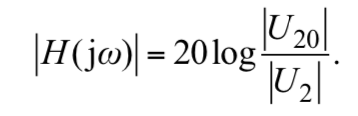
\includegraphics[width=5cm]{def_insertionloss.png}
	\caption{insertionloss}
	\label{fig:insertion loss}
\end{figure}
Wobei H dem Streuparameter (S-Parameter) S index 21 entspricht. Die Einfügungsverluste sind auch mit dem Verhältnis von eingehenden zu abegegebenen Leistung zu Berechnen, jedoch eignet sich diese Methode mehr beim messtechnischen bestimmen der Einfügungsverluste. Da die Berechnungen in einem Bereich von bis zu 30 MHz gemacht werden, ist es notwendig die parasitären Parameter von Spule und Kondensator miteinzubeziehen. Zudem können sie in einem Bereich von +- 30% vaariert werden.

\subsection{Schaltungen} \label{subsec:schaltungen}
CM:
\begin{figure}[H]
	\centering
	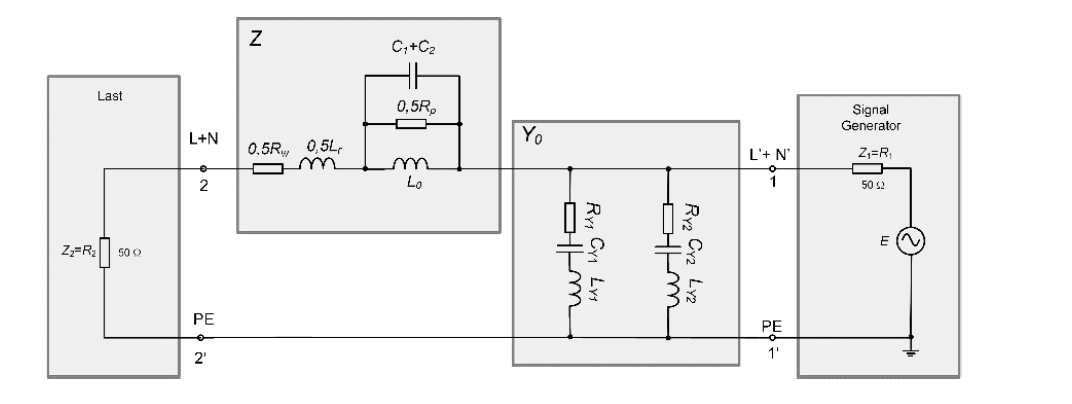
\includegraphics[width=15cm]{CM_ElectricalCircuit.png}
	\caption{CM-Schaltungäquvalent}
	\label{fig:CM-Schaltungäquvalent}
\end{figure}
DM:
\begin{figure}[H]
	\centering
	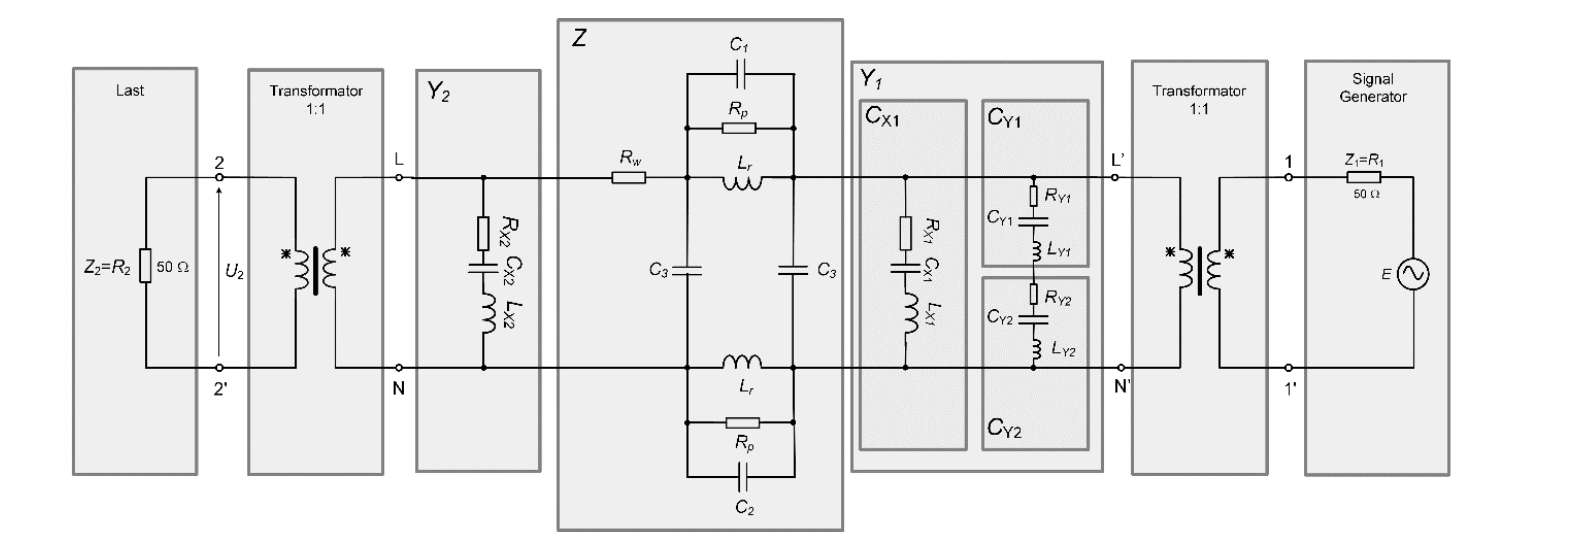
\includegraphics[width=15cm]{DM_ElectricalCircuit.png}
	\caption{DM-Schaltungsäquvalent}
	\label{fig:DM-Schaltungsäquvalent}
\end{figure}
\subsection{Vorgehen} \label{subsec:vorgehen}
Die Einfügungsverluste werden analytisch ermittelt. Im ersten Schritt werden die Berechnungen in MATLAB gemacht. Somit können die Funktionen eifach geplottet werden. Diese Plots werden dann mit Simulationen in MPLAB Mindi verglichen um festzustellen ob diese korrekt sind. Die vollständigen und korrekten Berechnungen können somit in Java implementiert werden. Um die Einfügungsverluste bestimmen zu können, wird das Model der 2-Tore verwendet. Einzelne Schaltungsteile werden in ABCD-Matrixen abgebildet, welche dann durch Kaskadierung der einzelnen ABCD-Matrixen zusammengeführt werden. Die Einfügungsverluste werden den S-Parameter abgeleitet, welche direkt aus der ABCD-Matrix errechnet werden kann.
Der S-Parameter Index 12 gibt den Tranmissionsgrad der Wellen an, die vom Tor 1 zum Tor2 übertragen wird. Die S-Parameter sind abhängig von den Bezugswiderständen (Innenwiderstand der Quelle sowie Lastwiderstand). In unserem Fall sind die Bezugswiderstände mit 50Ohm gegeben.

\newpage









